\lstinputlisting[language=bash,basicstyle=\small]{python_codes/fieldstone_110/keywords}

\begin{center}
Code at \url{https://github.com/cedrict/fieldstone/tree/master/python_codes/fieldstone_110}
\end{center}

\par\noindent\rule{\textwidth}{0.4pt}

%%%%%%%%%%%%%%%%%%%%%%%%%%%%%%%%%%%%%%%%%%%%%%%%%%%%%%%%%%%%%%%%%%%%%%%%%%%%%%%%%%%%%%%%%%%%%%%%%%%%

\index{general}{Boussinesq Approximation}
\index{general}{Extended Boussinesq Approximation}

The setup is taken from Blankenbach \etal (1989) \cite{blbc89} (See \stone 3, and Section~\ref{ss:blbc89}). 
The equations that we are solving are presented in Section~\ref{ss:dimeqs2}. 
Boundary conditions are free slip on all sides. There is therefore a pressure nullspace
so a normalisation condition is needed.
$Q_2\times Q_1$ elements are used here. 

Since we are only interested in the steady state and not the path to steady state, 
then the $\partial_t T$ term in the energy equation is zeroed and Picard iterations
are used (with a relaxation parameter of 0.5) to arrive at the steady state.
The convergence criterion is based on two factors: when the temperature field and the Nusselt number 
relative difference fall below the tolerance $tol=10^{-7}$ then iterations stop.
Note that the relaxation parameter can be close to 1 when the Rayleigh number is low.

The parameters are:
\[
L_x=L_y=1
\qquad
\alpha=2.5\cdot 10^{-3}
\qquad
k=1
\qquad
C_p=10^{-2}
\qquad
\rho_0=20
\qquad
T_0=0
\qquad
\vec{g}=(0,-1)
\qquad
\Delta T = 1
\]
The Rayleigh number $\Ranb$ is an input of the code ($10^4$, $10^5$ or $10^6$), so 
we choose the viscosity accordingly:
\[
\eta_0 = \frac{\alpha g_y L_y^3 \rho_0^2 C_p \Delta T}{k \Ranb}
\]
This choice of parameters yields the following dissipation number:
\[
\Dinb=\frac{\alpha g_y L_y}{C_p} = 0.25
\]
The Boussinesq Approximation only relies on the Rayleigh number but the 
Extended Boussinesq Approximation relies on both Rayleigh and Dissipation numbers\footnote{Note that 
the temperature at the surface is also necessary to define the setup in a unique manner. This observation
has been a major source of headache in efforts to replicate benchmark papers.}. 
Because we target this specific value of $\Dinb$ we could not choose the 
parameters entering the Rayleigh number as freely as before.

The shear heating term is $\Phi=2 \eta_0 \dot{\bm \varepsilon}:\dot{\bm \varepsilon}$ since the flow
is incompressible. With regards to solving the energy equation this term is trivial since it does not
depend on temperature at all.

The adiabatic term is $\alpha T \vec{\upnu}\cdot\vec\nabla p$. 
First we see that it depends on temperature so it should normally be discretised in such a 
way that it contributes to the FE matrix. However, since we are solving for the steady state
iteratively we decide to leave it as a rhs term.
The pressure is bilinear so its gradient at the quadrature points is easy to compute.  
Also because it is the gradient and not the pressure itself that enters this term then 
the normalisation constant does not influence results.
Note that this term is often linearised by assuming that the pressure is mostly hydrostatic
so that it then becomes: $- \alpha T \rho_0 \vec\upnu\cdot\vec{g}$.
Both expressions are exported to the vtu file for visual comparison.

Since no work is done on the domain and there are no heat sources/sinks, we then 
expect that energy conservation yields a zero heat flux balance on the boundary of the domain. 
Since no temperature is imposed on the sides this implies a zero heat flux. 
We can then monitor the bottom and top heat fluxes and sum them, expecting zero.  


As explained in Section~\ref{ss:dimeqs2}, the above choice of parameters yields the following 
fundamental reference quantities:
\begin{itemize}
\item a length $L_{ref}=1$ 
\item a temperature $T_{ref}=1$ 
\item a viscosity $\eta_{ref}=\eta_0=10^{-6,7,8}$ (corresponding to $\Ranb=10^{4,5,6}$) 
\item a thermal diffusion coefficient $\kappa_{ref}=k/\rho_0 C_p = 5$ 
\end{itemize}
and the derivative reference quantity $\upnu_{ref} = L_{ref} / t_{ref} = \kappa_{ref}/L_{ref} = 5$.
When written to file the root mean square velocity is divided by $\upnu_{ref}$ so as to allow
for a direct comparison with existing published values.
In what follows we monitor:
\begin{itemize}
\item the dimensionless root mean square velocity $\upnu_{rms}/\upnu_{ref}$
\item the average temperature $\langle T \rangle$
\item the dimensionless Nusselt number $\Nunb$
\item the heat flow balance $\vec{q}_{top}+\vec{q}_{bottom}$
\item the steady state average vertical temperature and velocity profiles
\end{itemize}

The way the code is written now means that resolution is limited to 80x80 elements 
because of the memory cost (approx. 30Gb).

Note that the \aspect results may not be true steady state, but the first 3 digits are good.

\newpage
%------------------------------------------------------------------------------
\subsection*{Boussinesq Approximation (BA)}

\begin{center}
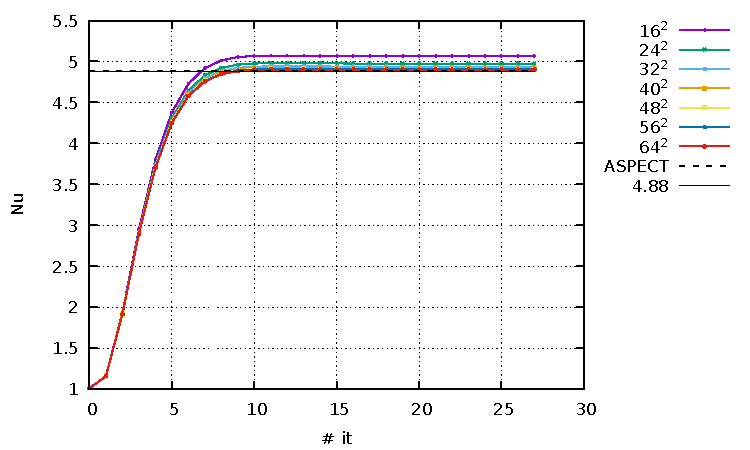
\includegraphics[width=5.7cm]{python_codes/fieldstone_110/results_BA/Nu_Ra1e4.pdf}
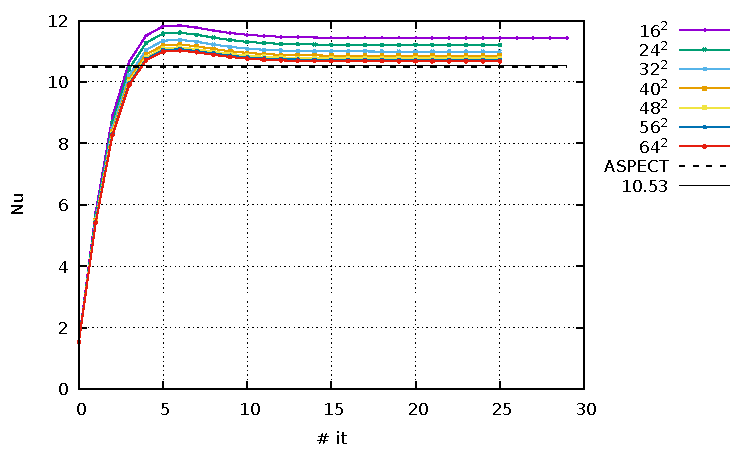
\includegraphics[width=5.7cm]{python_codes/fieldstone_110/results_BA/Nu_Ra1e5.pdf}
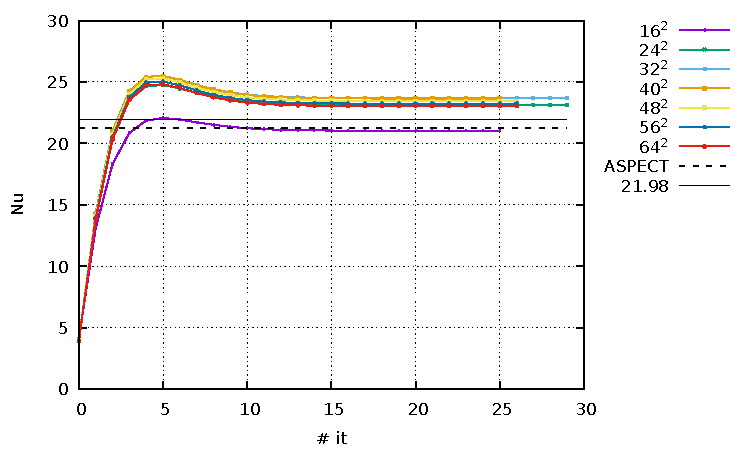
\includegraphics[width=5.7cm]{python_codes/fieldstone_110/results_BA/Nu_Ra1e6.pdf}\\
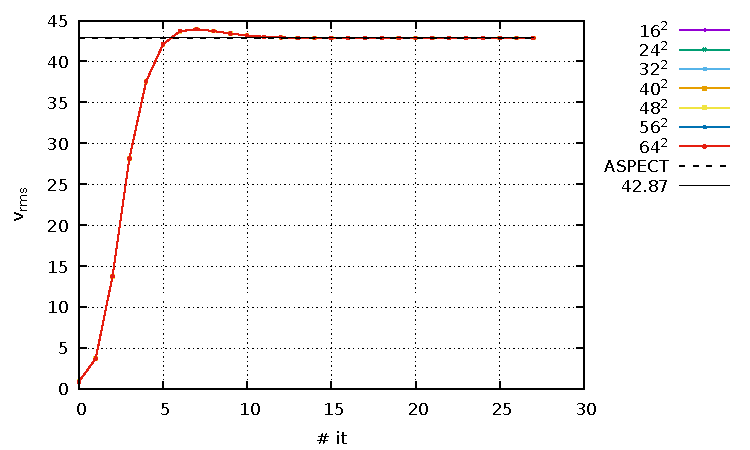
\includegraphics[width=5.7cm]{python_codes/fieldstone_110/results_BA/vrms_Ra1e4.pdf}
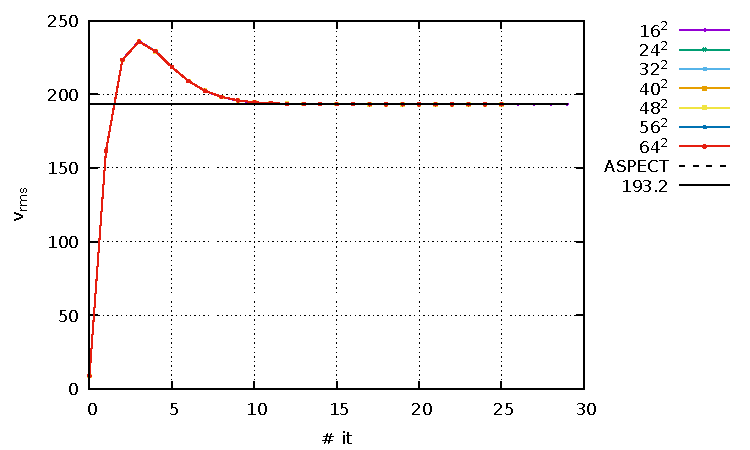
\includegraphics[width=5.7cm]{python_codes/fieldstone_110/results_BA/vrms_Ra1e5.pdf}
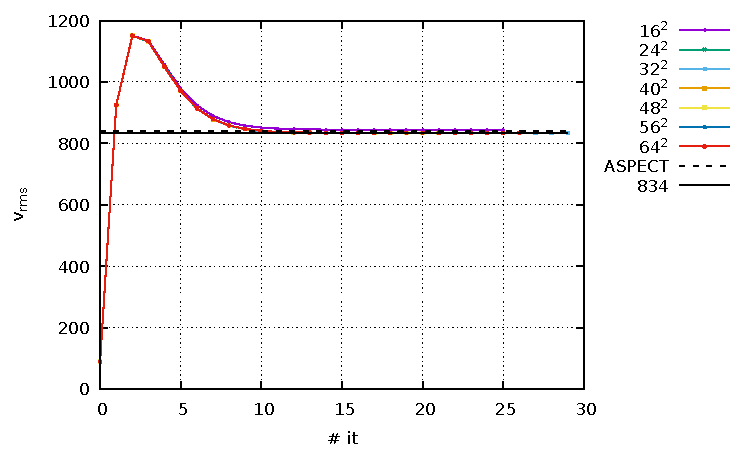
\includegraphics[width=5.7cm]{python_codes/fieldstone_110/results_BA/vrms_Ra1e6.pdf}\\
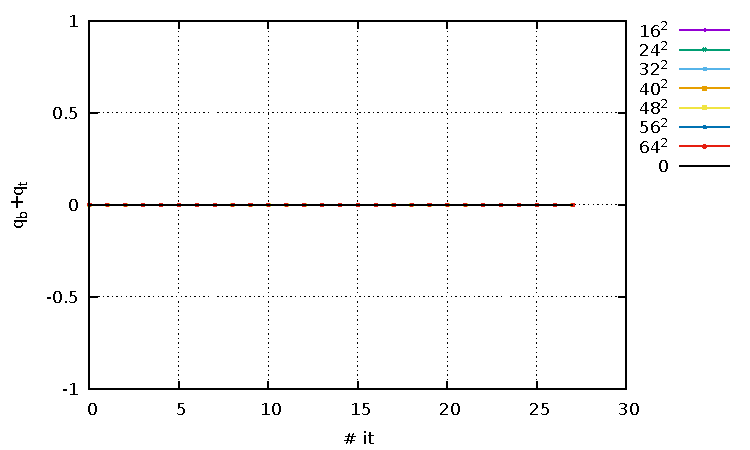
\includegraphics[width=5.7cm]{python_codes/fieldstone_110/results_BA/q_Ra1e4.pdf}
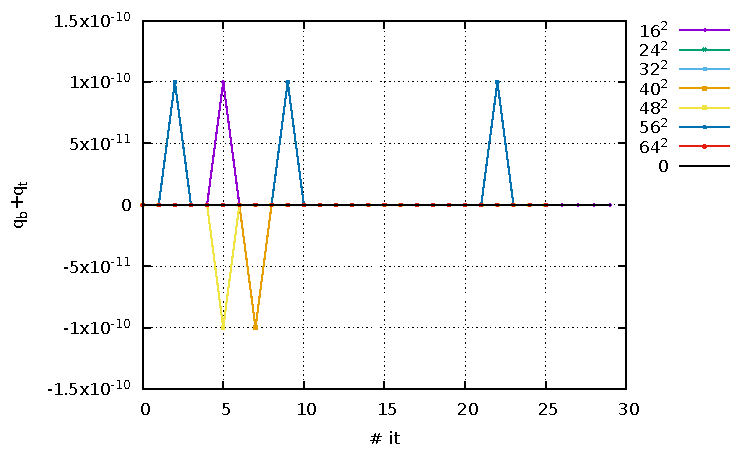
\includegraphics[width=5.7cm]{python_codes/fieldstone_110/results_BA/q_Ra1e5.pdf}
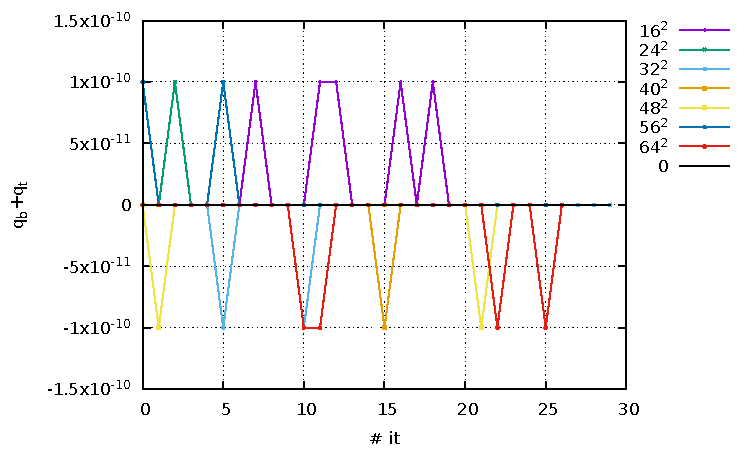
\includegraphics[width=5.7cm]{python_codes/fieldstone_110/results_BA/q_Ra1e6.pdf}\\
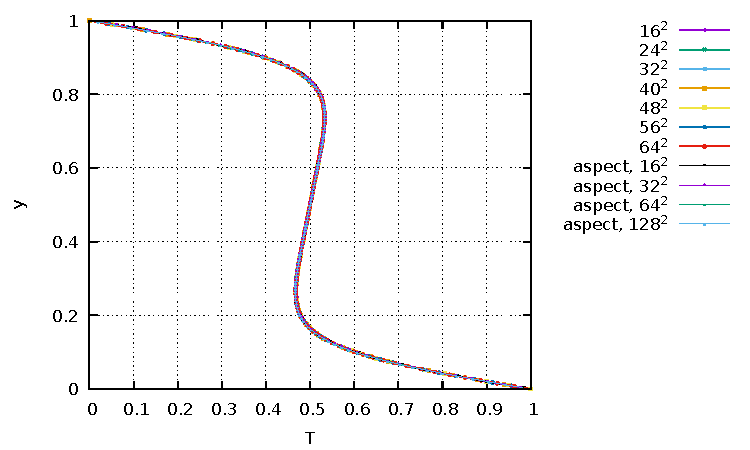
\includegraphics[width=5.7cm]{python_codes/fieldstone_110/results_BA/T_profile_Ra1e4.pdf}
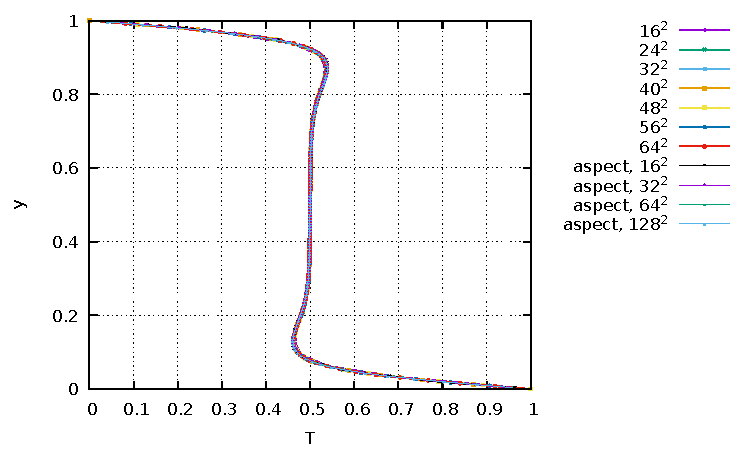
\includegraphics[width=5.7cm]{python_codes/fieldstone_110/results_BA/T_profile_Ra1e5.pdf}
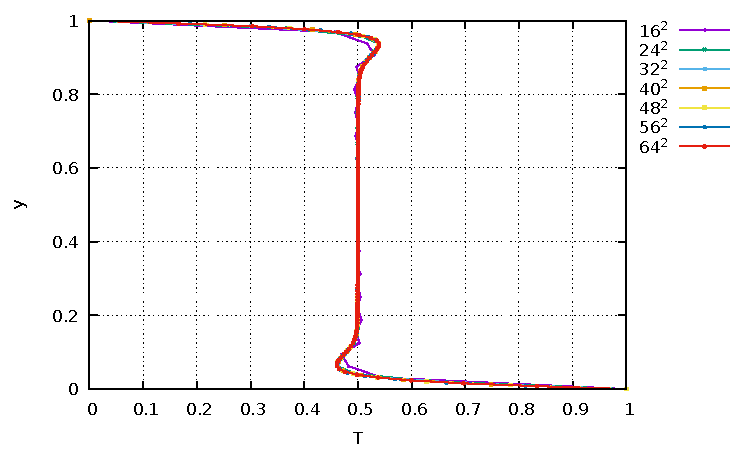
\includegraphics[width=5.7cm]{python_codes/fieldstone_110/results_BA/T_profile_Ra1e6.pdf}\\
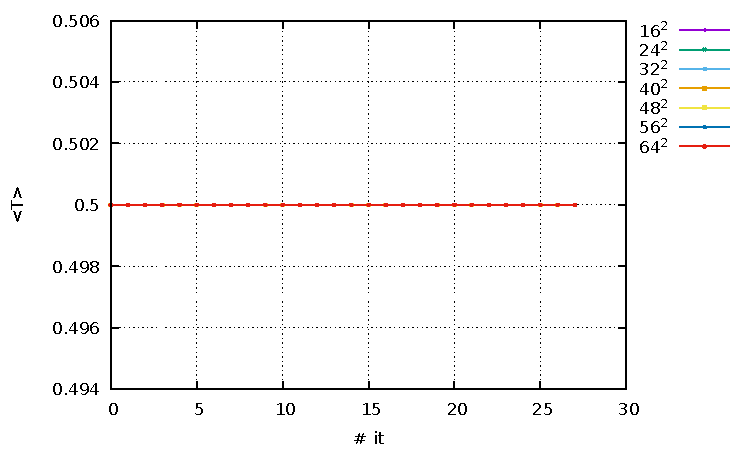
\includegraphics[width=5.7cm]{python_codes/fieldstone_110/results_BA/T_avrg_Ra1e4.pdf}
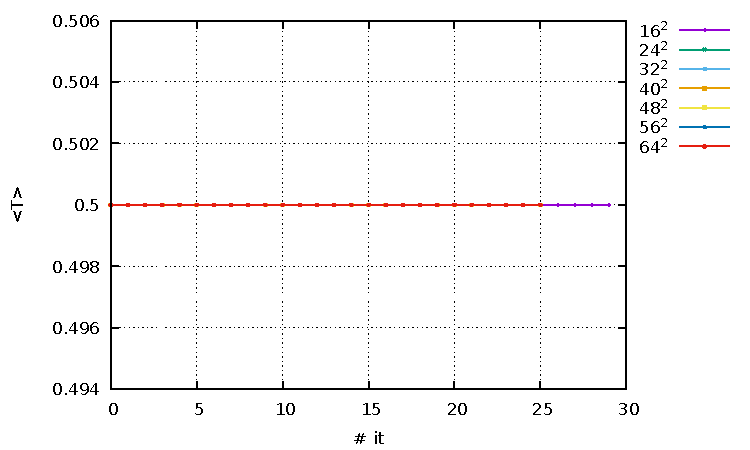
\includegraphics[width=5.7cm]{python_codes/fieldstone_110/results_BA/T_avrg_Ra1e5.pdf}
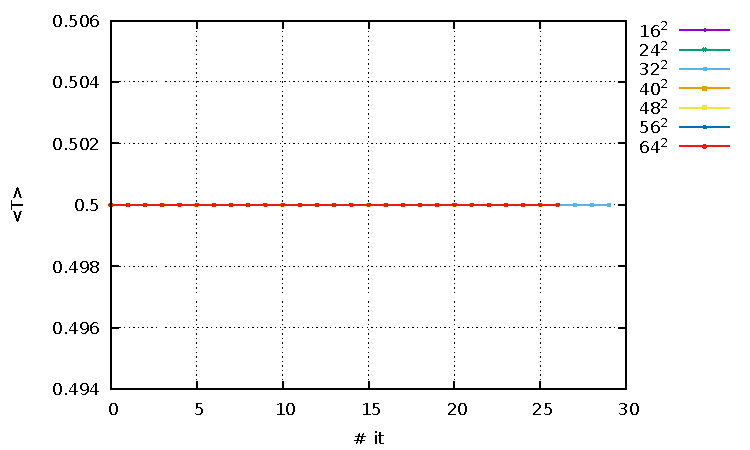
\includegraphics[width=5.7cm]{python_codes/fieldstone_110/results_BA/T_avrg_Ra1e6.pdf}\\
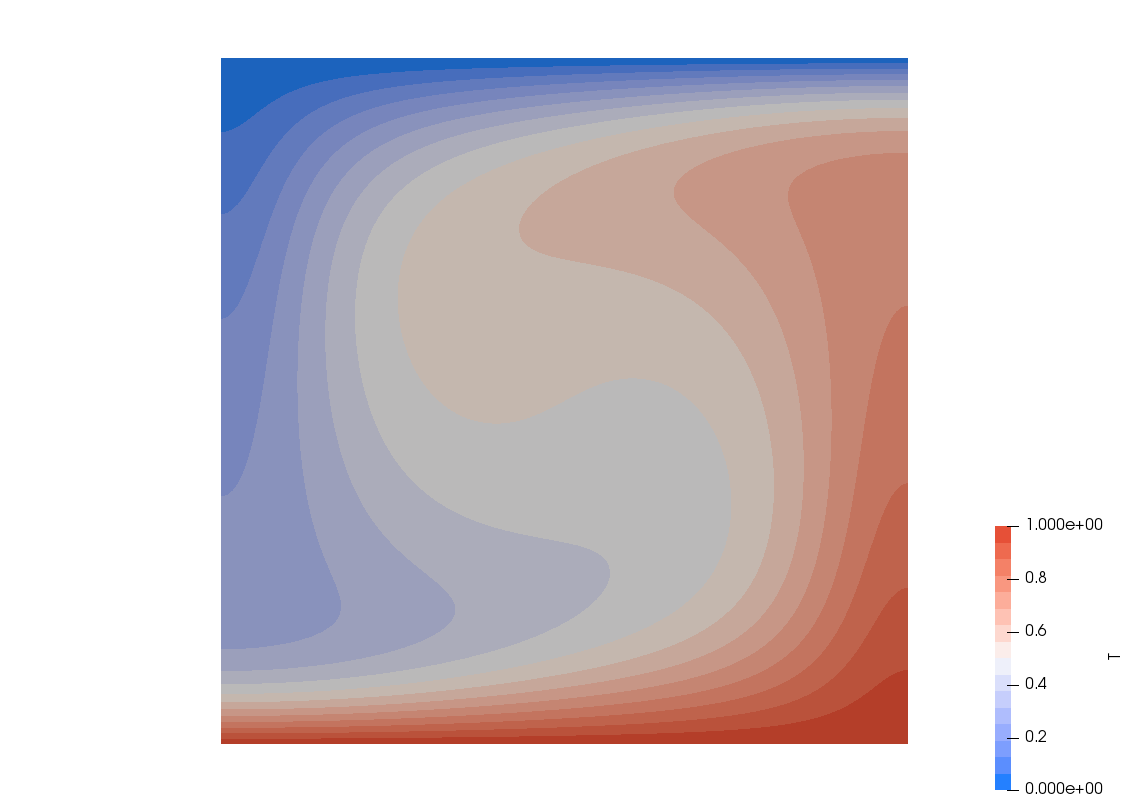
\includegraphics[width=5.7cm]{python_codes/fieldstone_110/results_BA/T_Ra1e4.png}
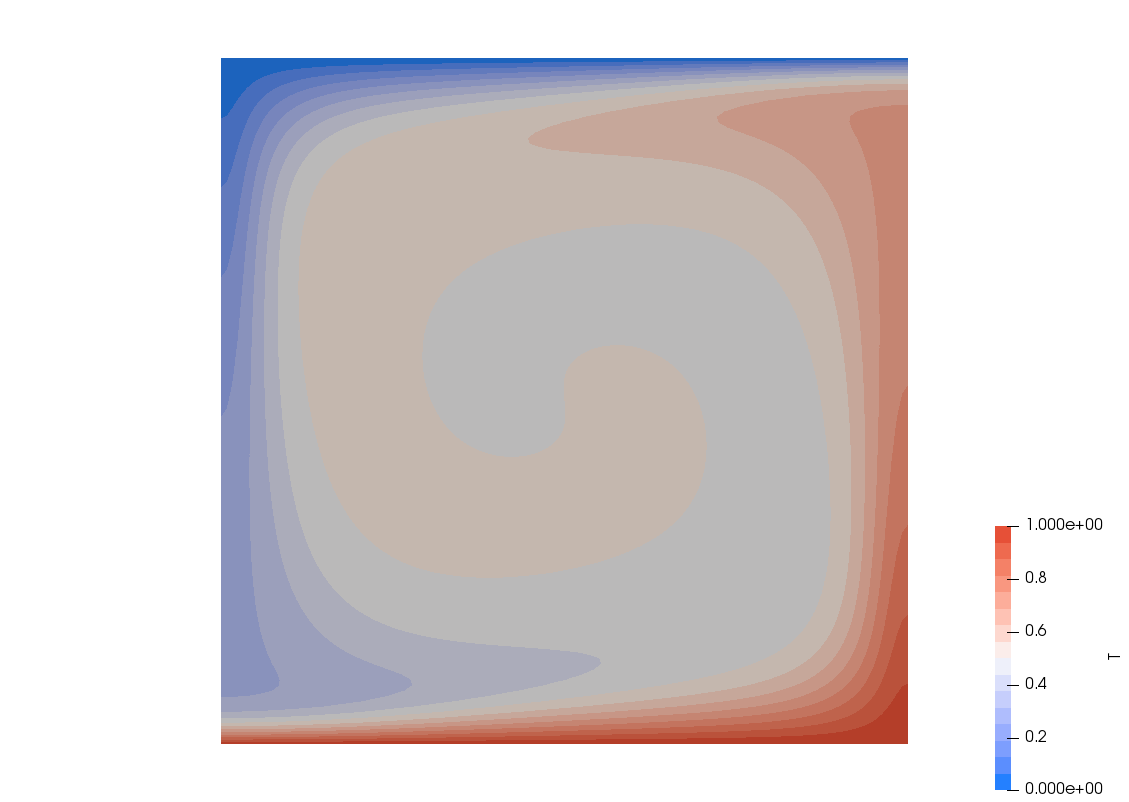
\includegraphics[width=5.7cm]{python_codes/fieldstone_110/results_BA/T_Ra1e5.png}
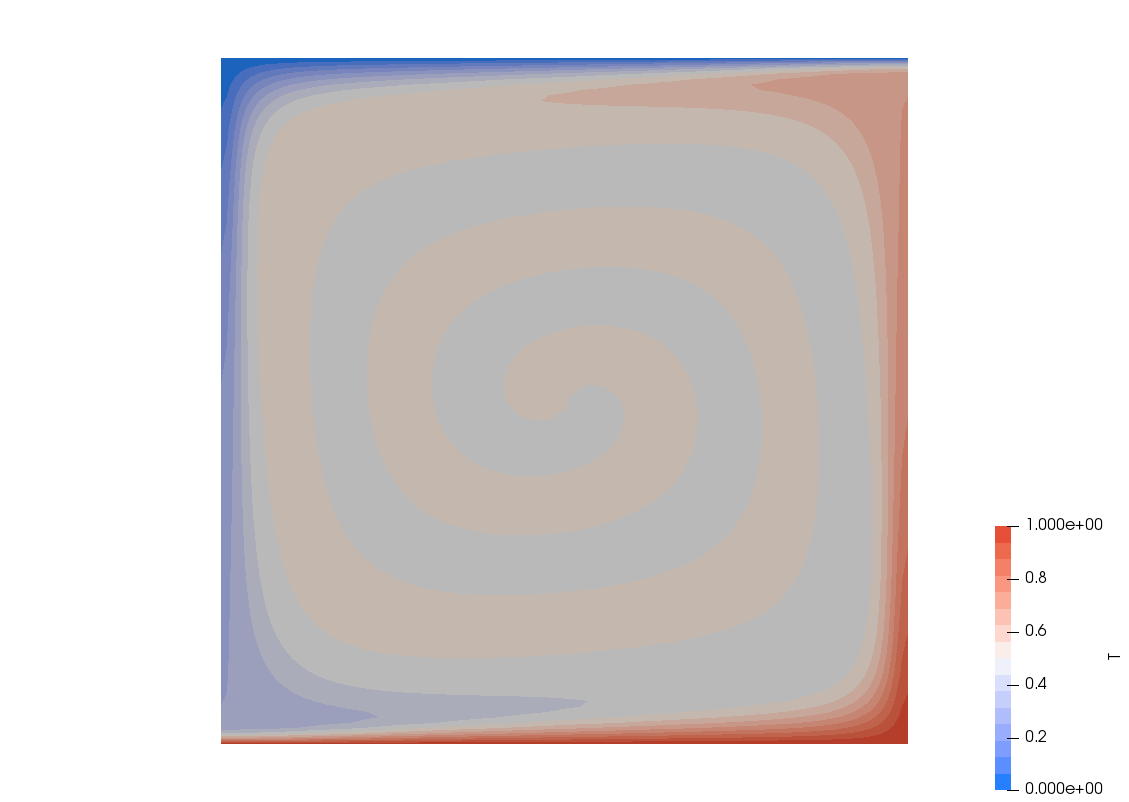
\includegraphics[width=5.7cm]{python_codes/fieldstone_110/results_BA/T_Ra1e6.png}\\
{\captionfont Left: $\Ranb=10^4$, middle: $\Ranb=10^5$, right: $\Ranb=10^6$} 
\end{center}

\newpage
\aspect results for 16x16 and 32x32 meshes

\begin{center}
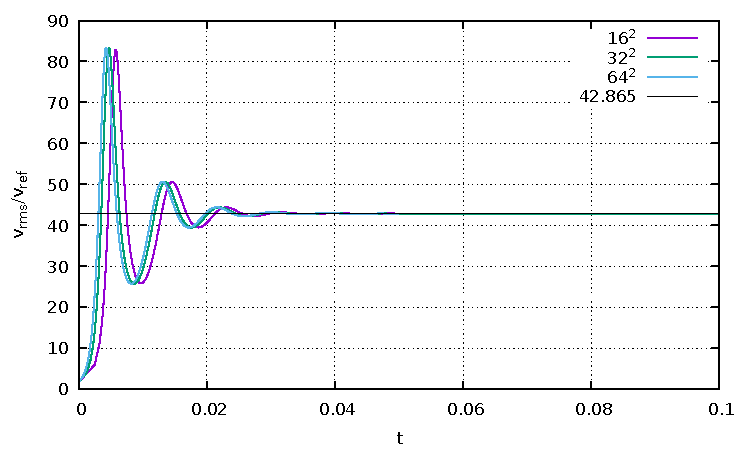
\includegraphics[width=5.7cm]{python_codes/fieldstone_110/results_BA/aspect/vrms_1e4}
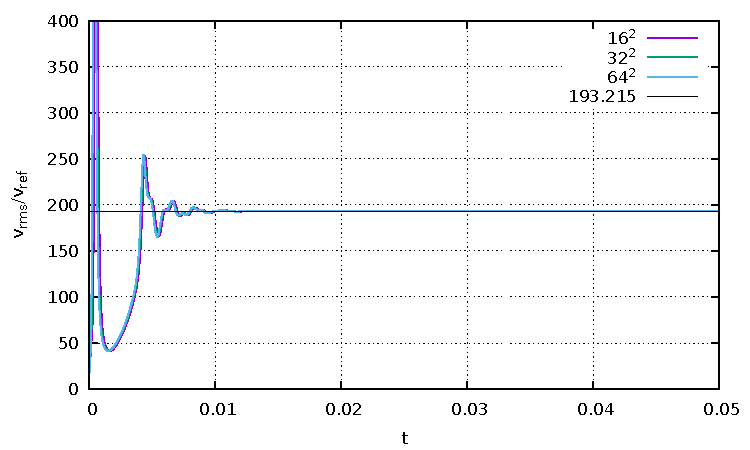
\includegraphics[width=5.7cm]{python_codes/fieldstone_110/results_BA/aspect/vrms_1e5}
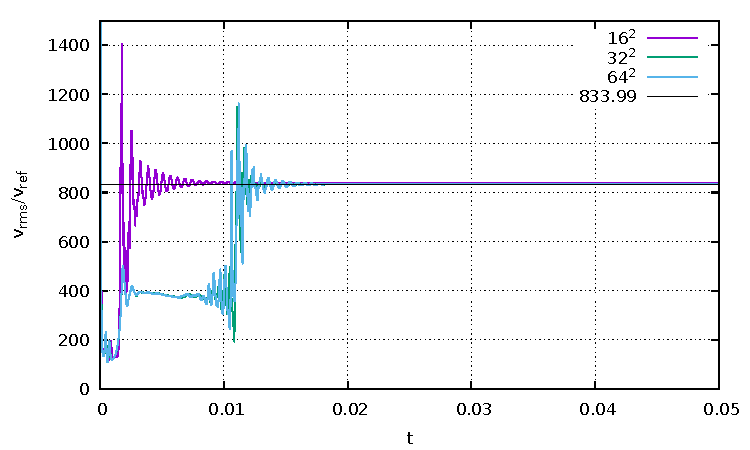
\includegraphics[width=5.7cm]{python_codes/fieldstone_110/results_BA/aspect/vrms_1e6}\\
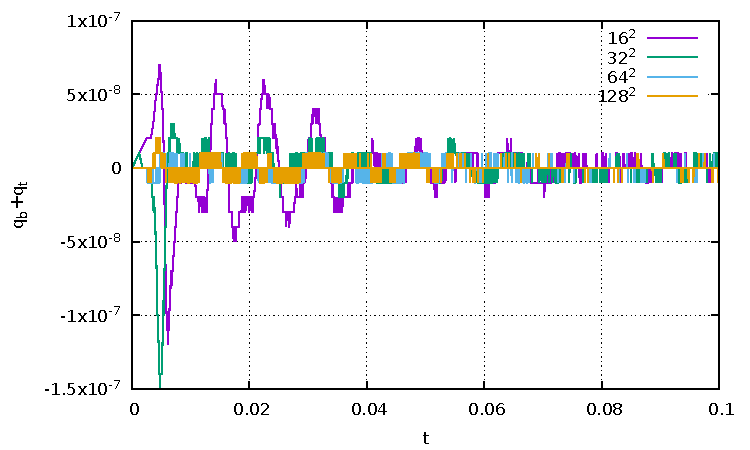
\includegraphics[width=5.7cm]{python_codes/fieldstone_110/results_BA/aspect/qsum_1e4}
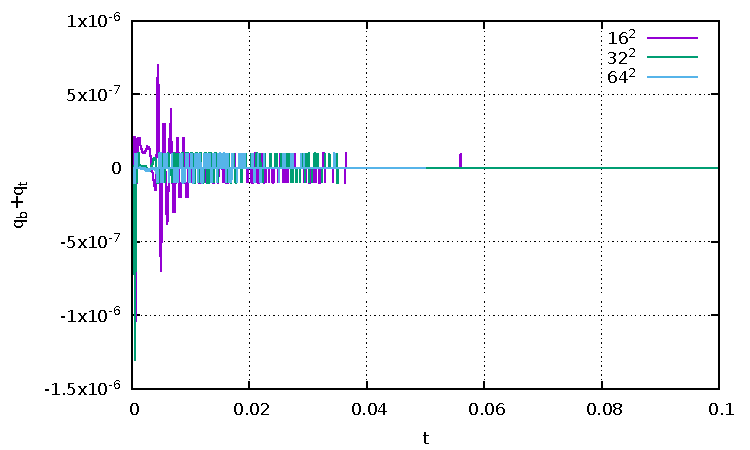
\includegraphics[width=5.7cm]{python_codes/fieldstone_110/results_BA/aspect/qsum_1e5}
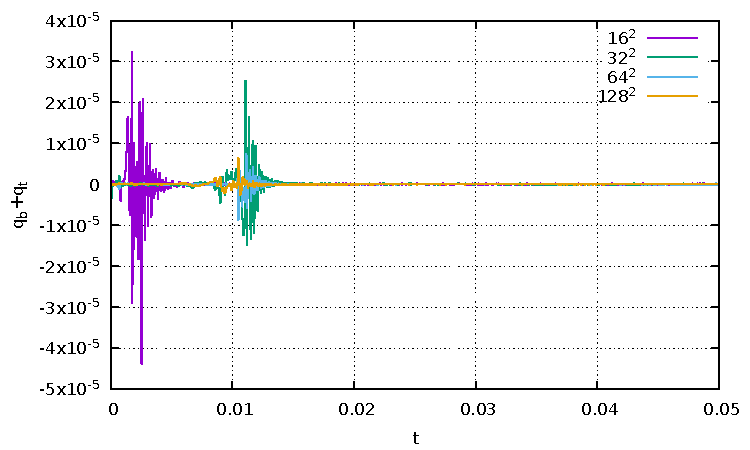
\includegraphics[width=5.7cm]{python_codes/fieldstone_110/results_BA/aspect/qsum_1e6}\\
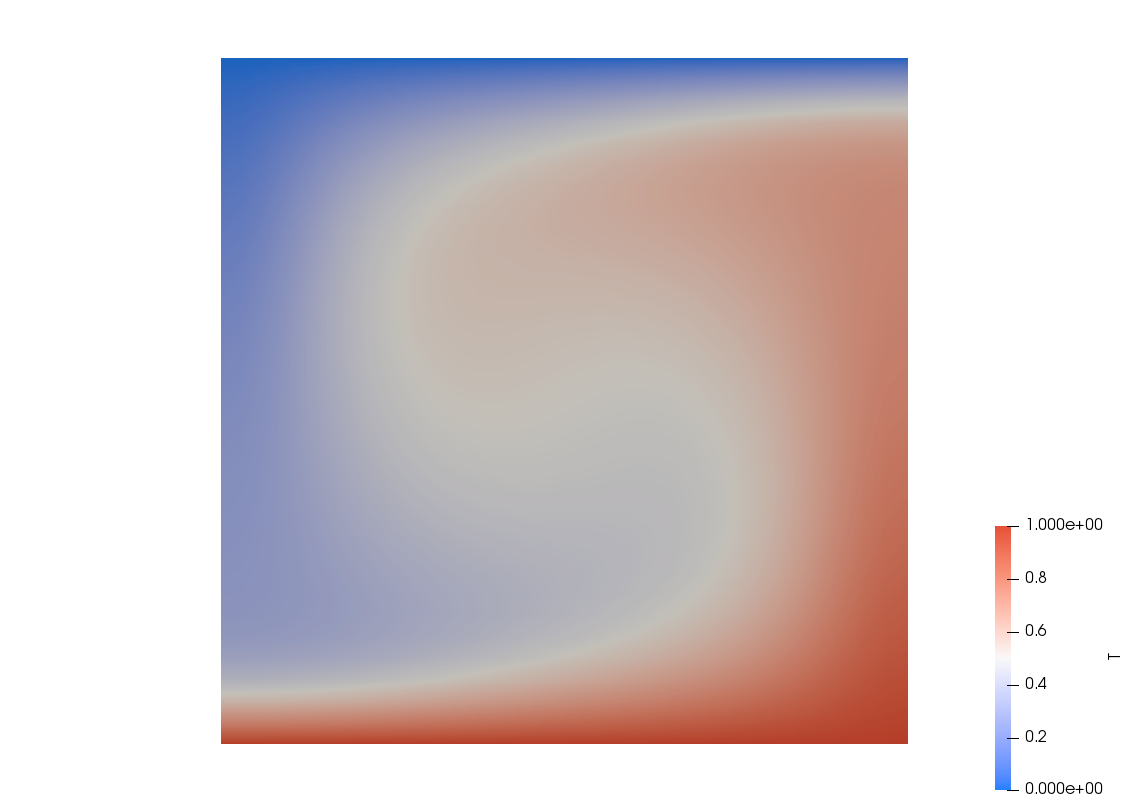
\includegraphics[width=5.7cm]{python_codes/fieldstone_110/results_BA/aspect/T_Ra1e4}
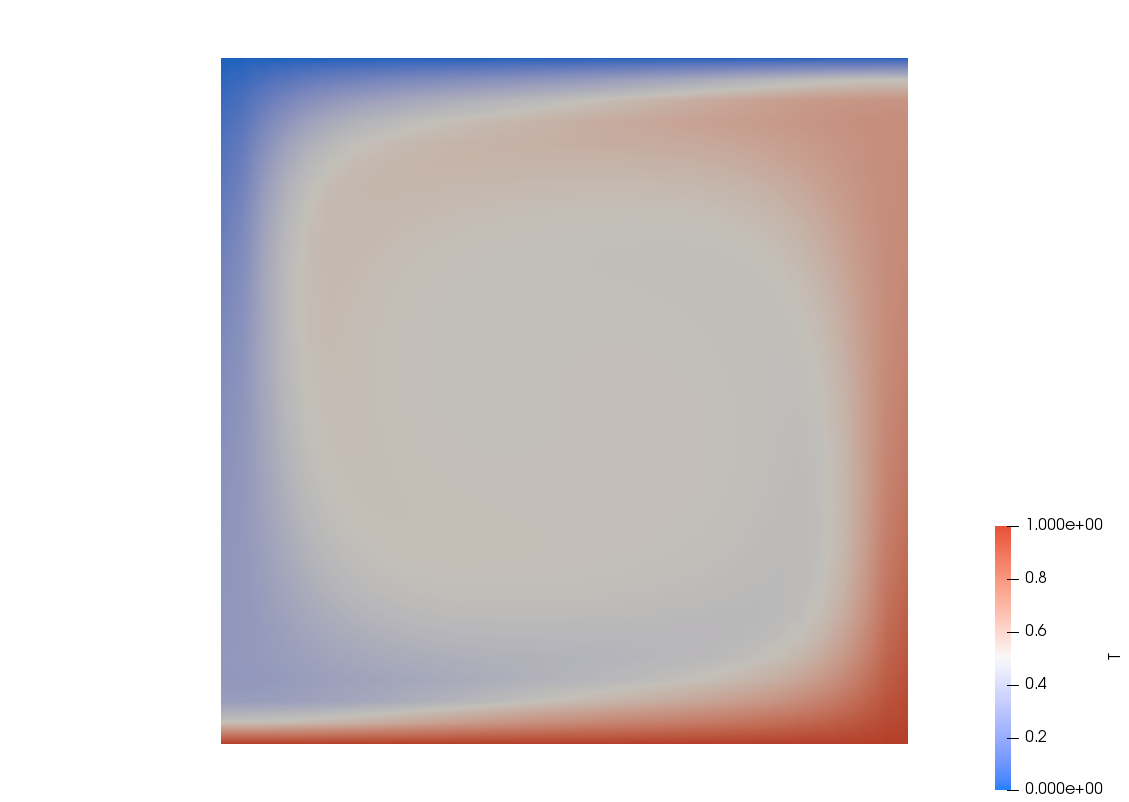
\includegraphics[width=5.7cm]{python_codes/fieldstone_110/results_BA/aspect/T_Ra1e5}
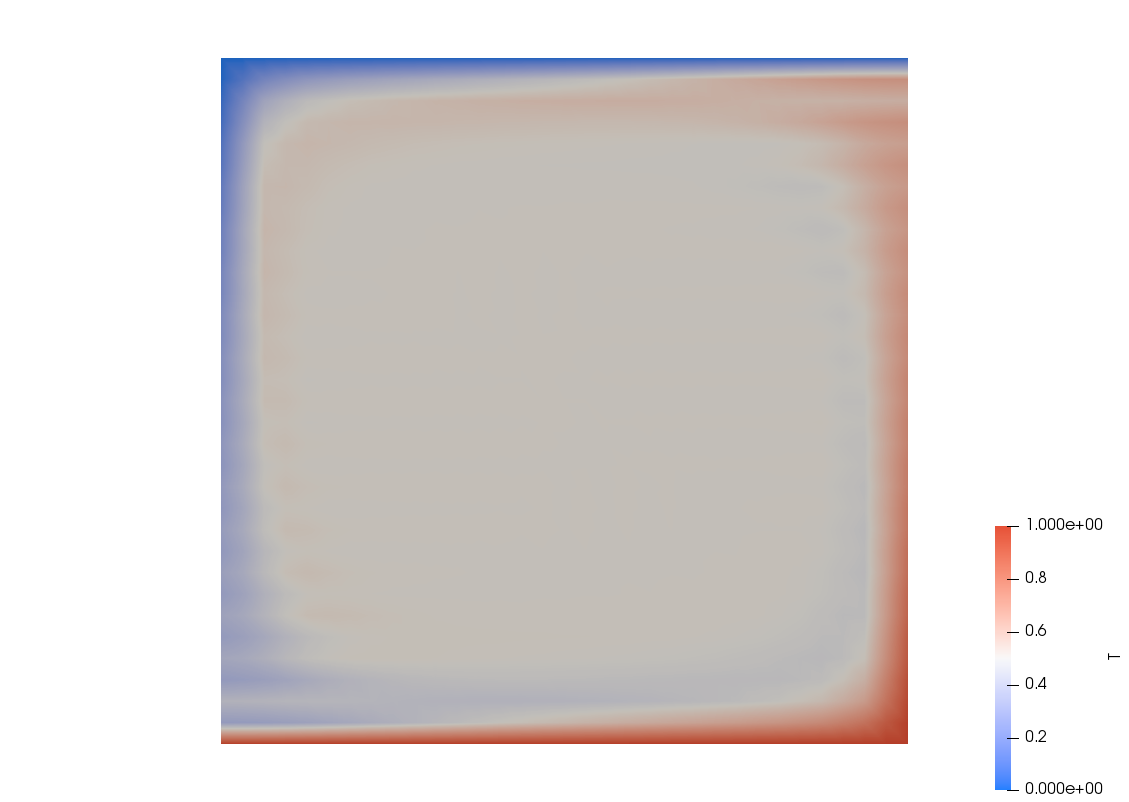
\includegraphics[width=5.7cm]{python_codes/fieldstone_110/results_BA/aspect/T_Ra1e6}\\
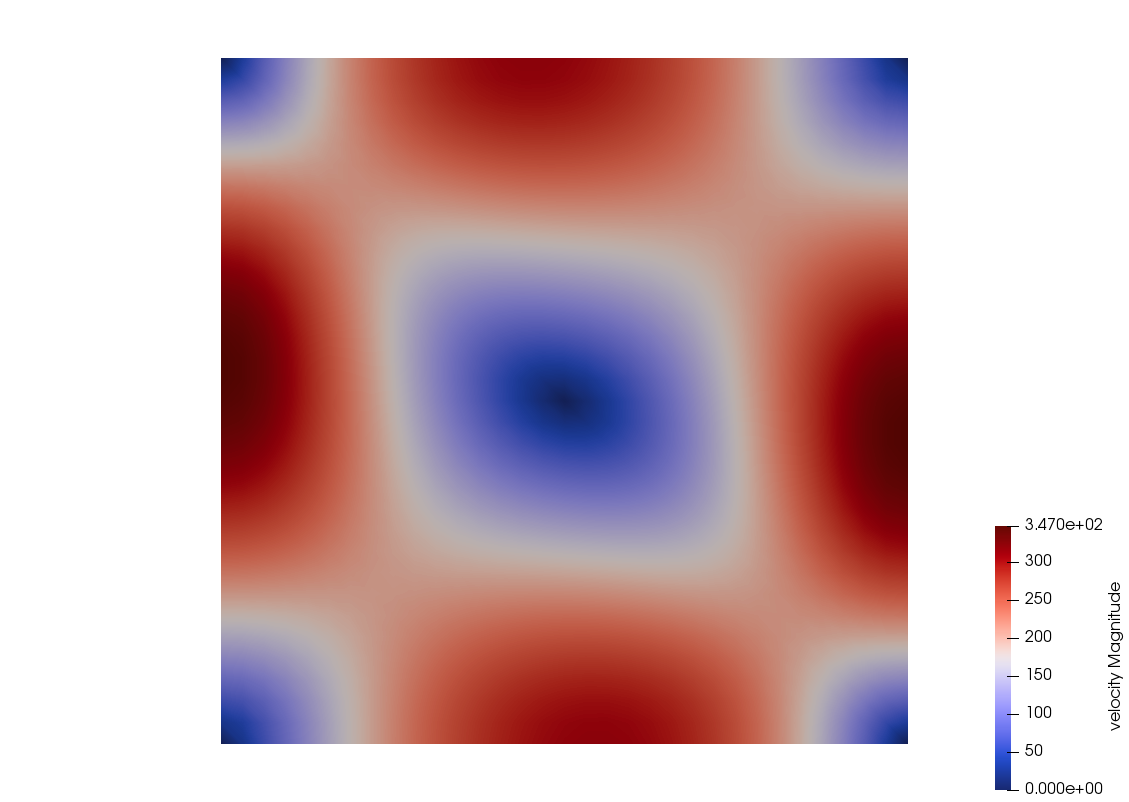
\includegraphics[width=5.7cm]{python_codes/fieldstone_110/results_BA/aspect/vel_Ra1e4}
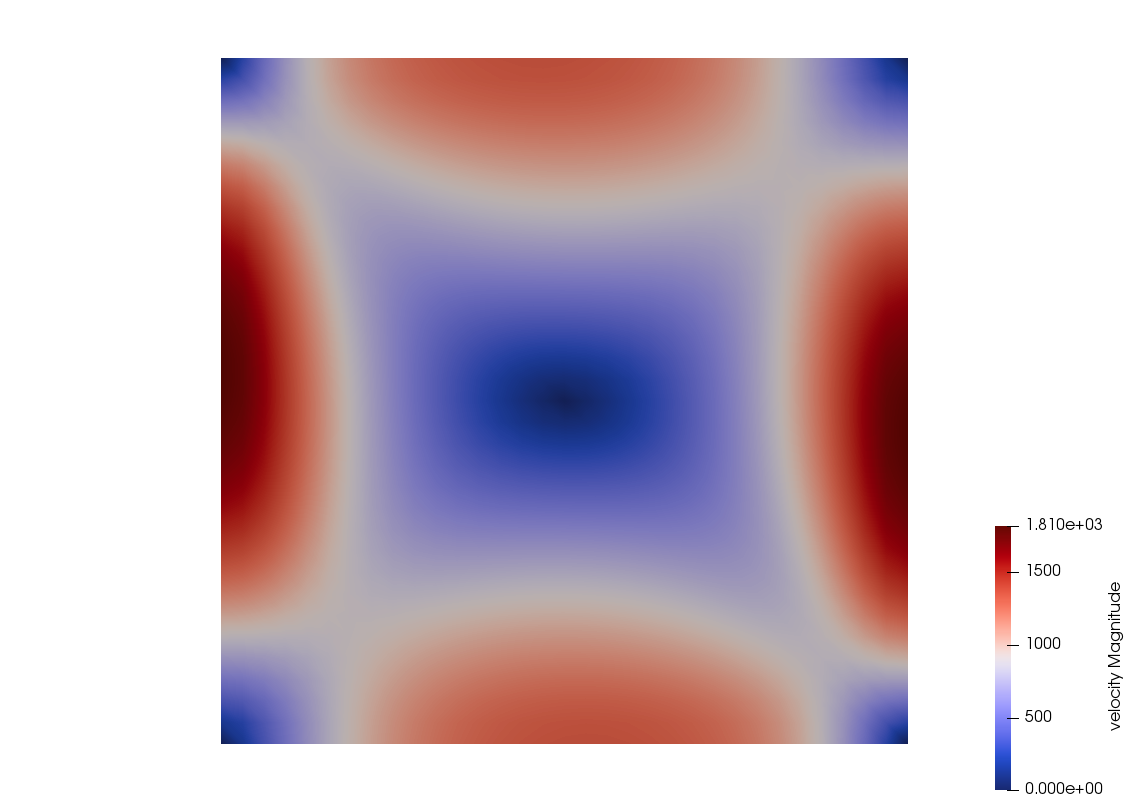
\includegraphics[width=5.7cm]{python_codes/fieldstone_110/results_BA/aspect/vel_Ra1e5}
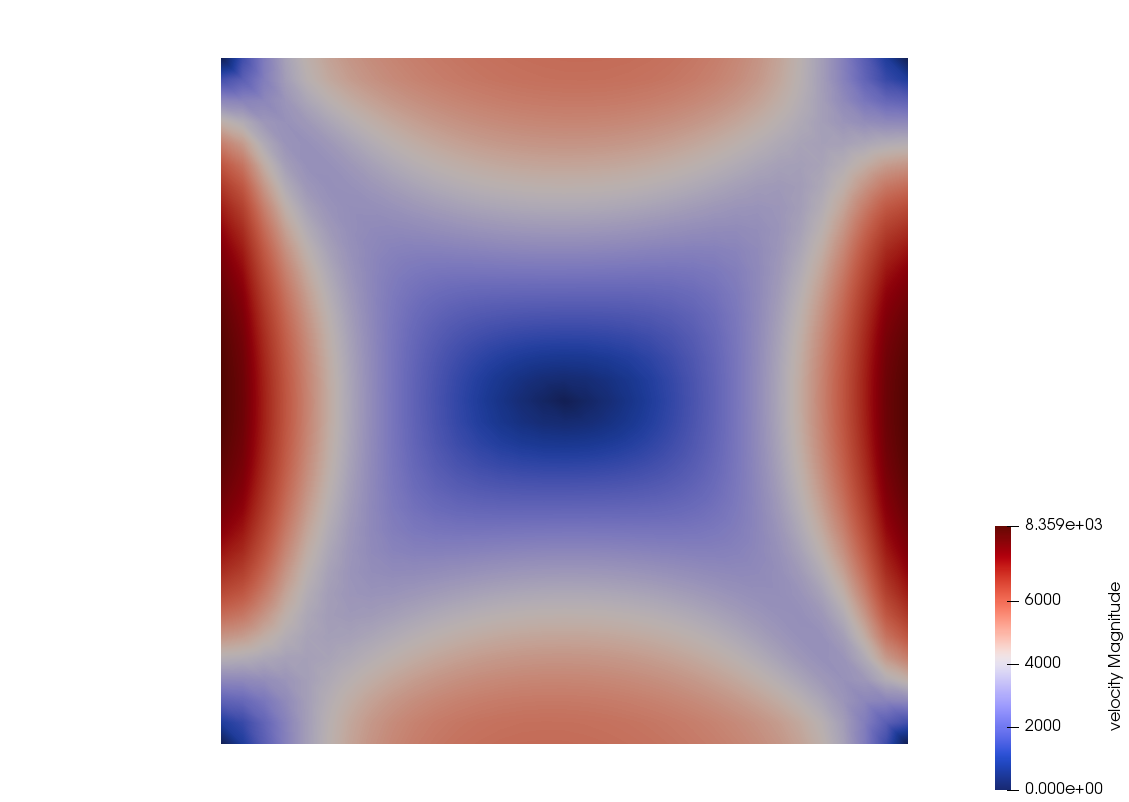
\includegraphics[width=5.7cm]{python_codes/fieldstone_110/results_BA/aspect/vel_Ra1e6}\\
{\captionfont Left: $\Ranb=10^4$, middle: $\Ranb=10^5$, right: $\Ranb=10^6$} 
\end{center}

\vspace{5mm}

\begin{center}
\begin{tabular}{llcccccc}
\hline
$\Ranb$  &  &\aspect  &\aspect  & \aspect & \stone 110  & \stone 110 & Blankenbach  \\
         &  &(16x16)  & (32x32) & (64x64) & (32x32)     & (64x64)    & \etal (1989) \\
\hline
\hline
$10^4$ & $\upnu_{rms}$ &  42.8656918  & 42.865026   & 42.8627448  & 42.8650211917 & 42.8649453947 & 42.864947   \\
       & $q_{bot}$     &  -4.88459727 & -4.88443000 & -4.88484574 & -4.9371243062 & -4.8980781972 & 4.884409 \\
       & $q_{top}$     &  +4.88459726 & +4.88443000 & +4.88484574 & +4.9371243062 & +4.8980781972 &  \\ 
\hline
$10^5$ & $\upnu_{rms}$ & 193.087842   & 193.214561  & 193.2147926 & 193.2144168167 & 193.2146484435 & 193.21454 \\ 
       & $q_{bot}$     & -10.4951125  & -10.5340940 & -10.5341271 & -10.9901799691 & -10.6715594312 & 10.534095 \\
       & $q_{top}$     & +10.4951125e & +10.5340940 & +10.5341271 & +10.9901799691 & +10.6715594312 &  \\
\hline
$10^6$ & $\upnu_{rms}$ & 839.48771    & 833.32106   & 833.972142  & 833.3211308177 & 833.9721673108 & 833.98977 \\
       & $q_{bot}$     & -21.2315844  & -21.8584326 & -2.19710401 & -23.6879005419 & -23.0372569642 & 21.972465 \\
       & $q_{top}$     & +21.2315844  & +21.8584327 & +2.19710400 & +23.6879005419 & +23.0372569642 &  \\
\hline
\end{tabular}\\
{\captionfont Velocity values are dimensionless in order to compare with Blankenbach \etal (1989)
but not the heat flux values.}
\end{center}

It looks like the heat flux calculations are much more accurate in \aspect, most likely 
due to the CBF algorithm. Also \aspect relies on the entropy stabilisation for the 
advection and it is likely to slightly alter the temperature field (additional diffusion
in zones of high gradients).


\newpage
On the following figures I report the steady state $\upnu_{rms}$ and $q_{top}$ 
values for both codes and for all three Rayleigh numbers:


\begin{center}
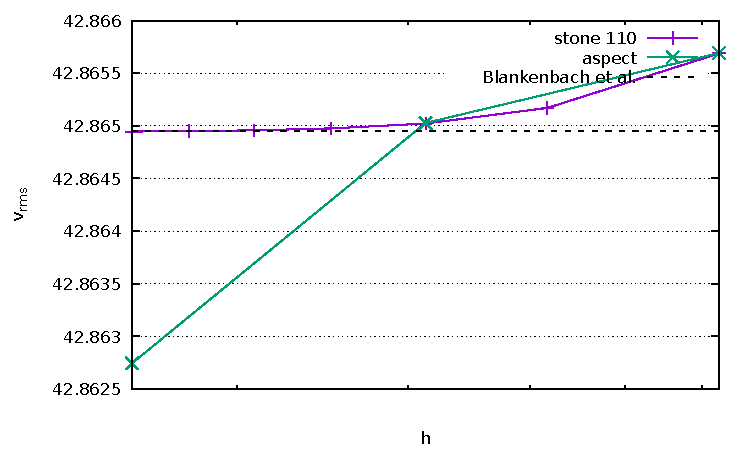
\includegraphics[width=5.7cm]{python_codes/fieldstone_110/results_BA/slopes/vrms_1e4}
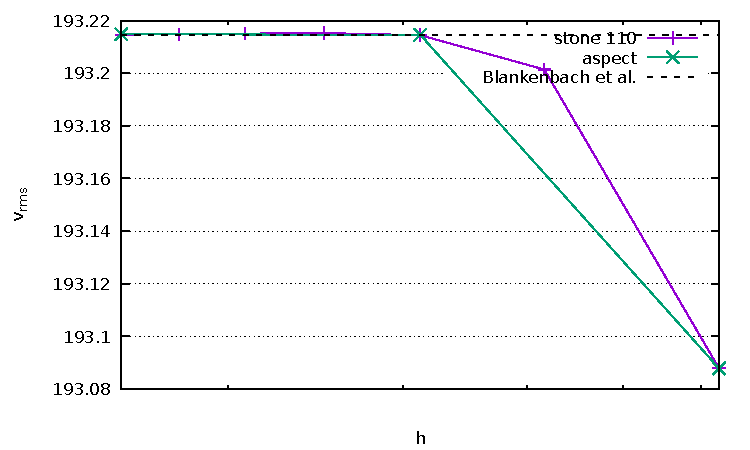
\includegraphics[width=5.7cm]{python_codes/fieldstone_110/results_BA/slopes/vrms_1e5}
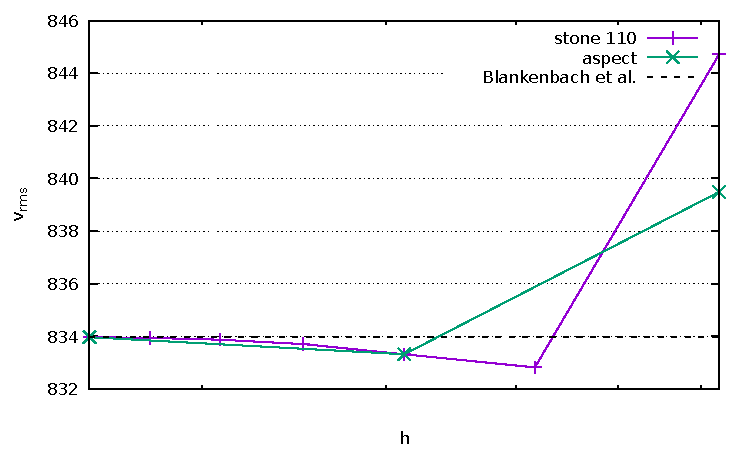
\includegraphics[width=5.7cm]{python_codes/fieldstone_110/results_BA/slopes/vrms_1e6}\\
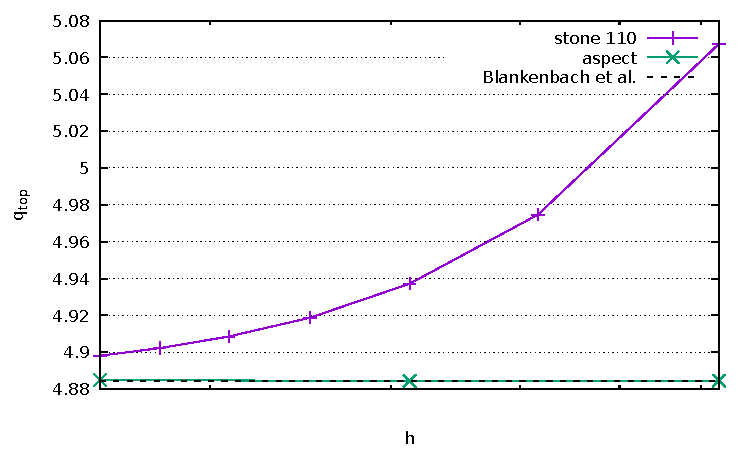
\includegraphics[width=5.7cm]{python_codes/fieldstone_110/results_BA/slopes/q_1e4}
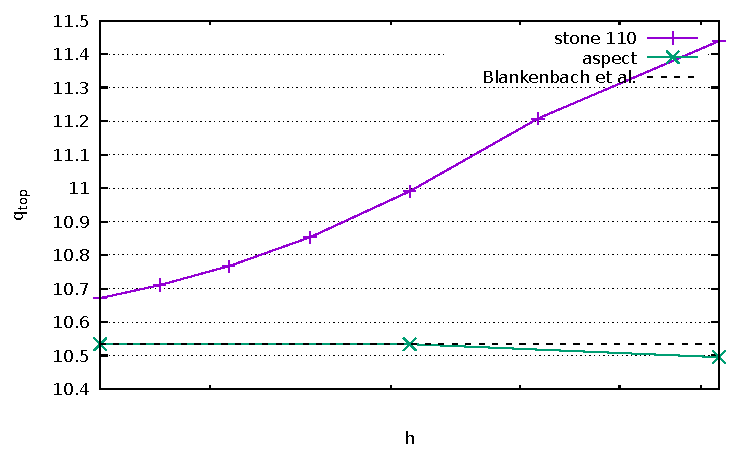
\includegraphics[width=5.7cm]{python_codes/fieldstone_110/results_BA/slopes/q_1e5}
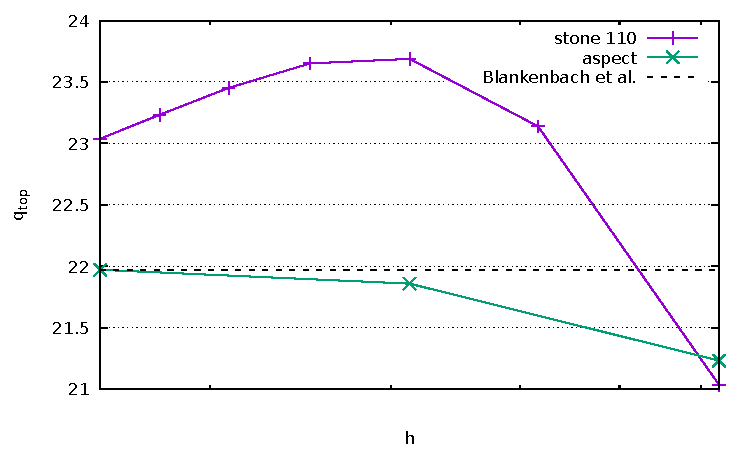
\includegraphics[width=5.7cm]{python_codes/fieldstone_110/results_BA/slopes/q_1e6}\\
{\captionfont Left: $\Ranb=10^4$, middle: $\Ranb=10^5$, right: $\Ranb=10^6$} 
\end{center}

The heat flux/Nusselt number results obtained with this \stone seem to converge 
to the expected values but \aspect results are much more accurate even at low
resolution... 
Looking at the vtu files they look virtually identical. since the vrms are also 
near identical I am def leaning towards the CBF for the reason why aspect$>$stone.

\begin{center}
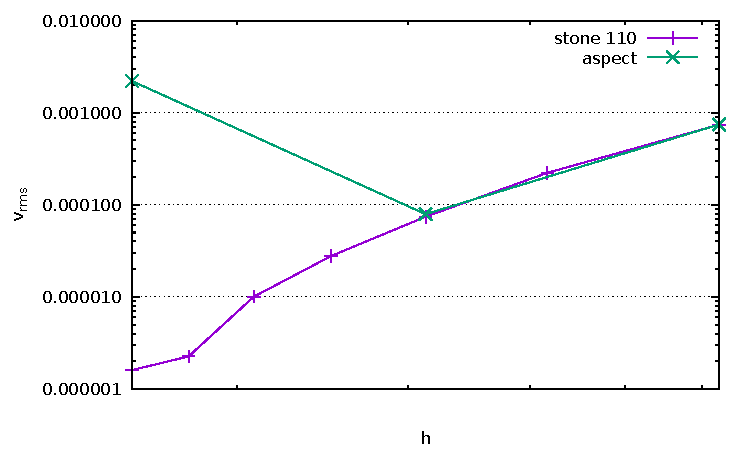
\includegraphics[width=5.7cm]{python_codes/fieldstone_110/results_BA/slopes/vrms_1e4_conv}
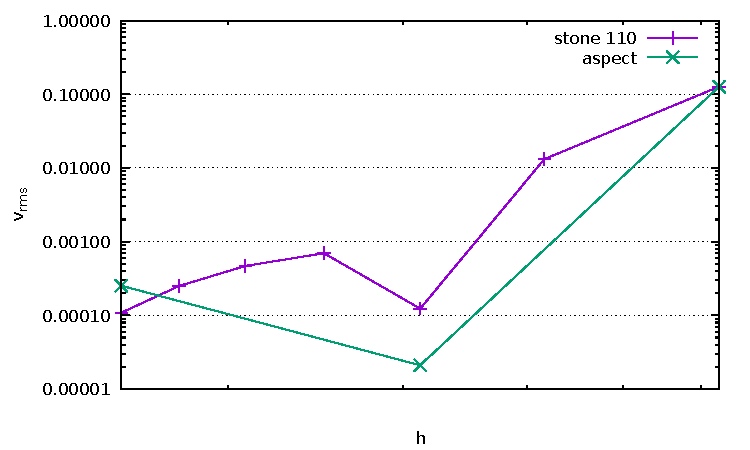
\includegraphics[width=5.7cm]{python_codes/fieldstone_110/results_BA/slopes/vrms_1e5_conv}
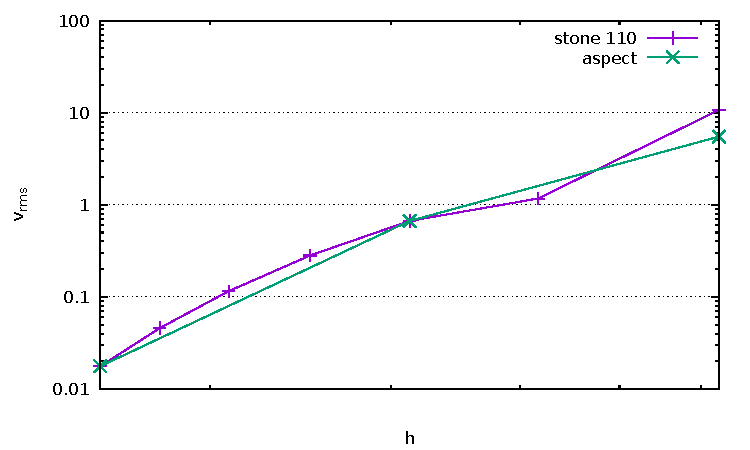
\includegraphics[width=5.7cm]{python_codes/fieldstone_110/results_BA/slopes/vrms_1e6_conv}\\
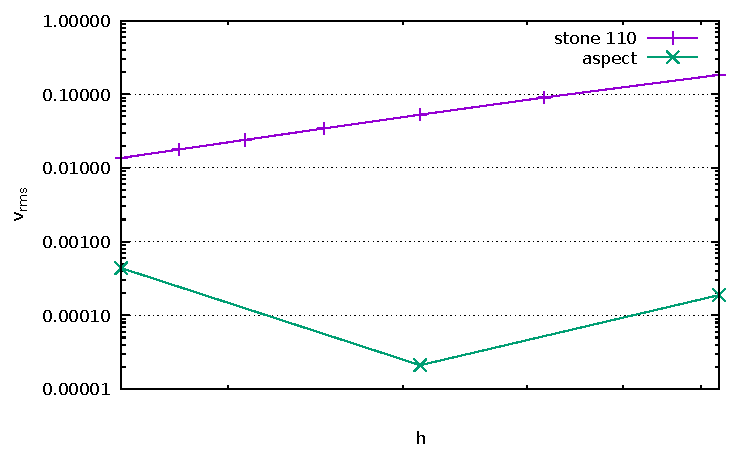
\includegraphics[width=5.7cm]{python_codes/fieldstone_110/results_BA/slopes/q_1e4_conv}
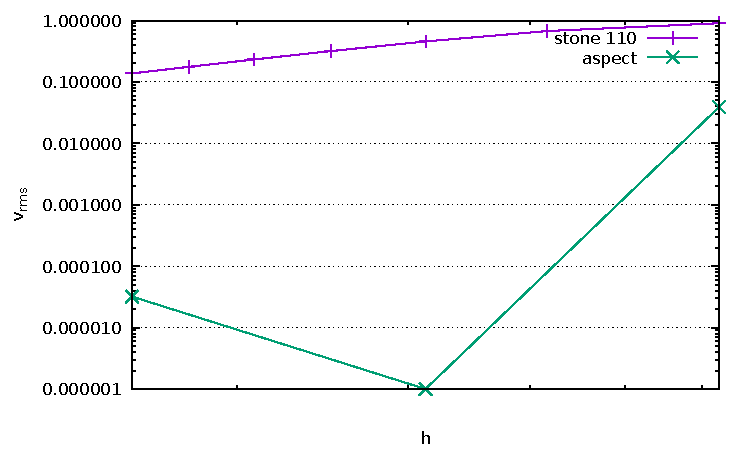
\includegraphics[width=5.7cm]{python_codes/fieldstone_110/results_BA/slopes/q_1e5_conv}
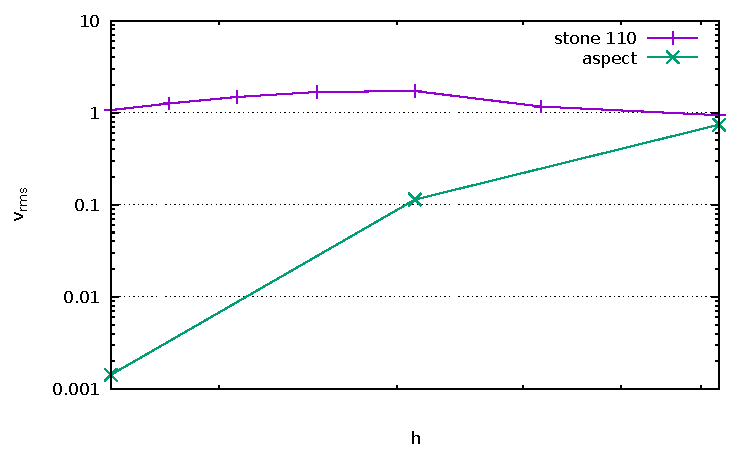
\includegraphics[width=5.7cm]{python_codes/fieldstone_110/results_BA/slopes/q_1e6_conv}\\
{\captionfont Left: $\Ranb=10^4$, middle: $\Ranb=10^5$, right: $\Ranb=10^6$} 
\end{center}


\newpage
%----------------------------------------------------------------
\subsection*{Extended Boussinesq Approximation (EBA)}

\begin{center}
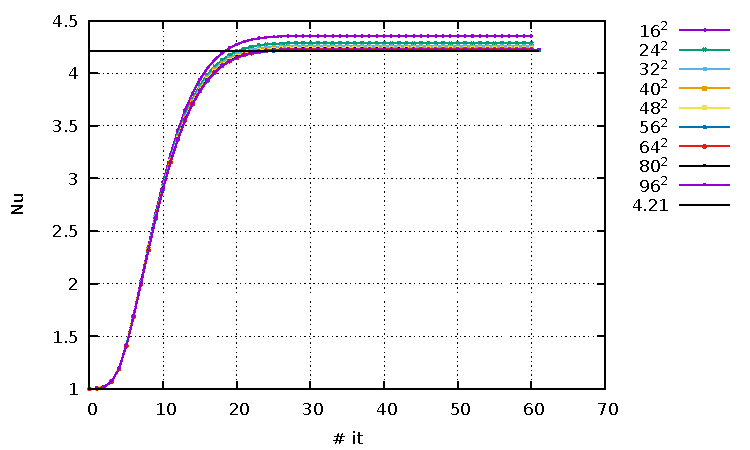
\includegraphics[width=5.7cm]{python_codes/fieldstone_110/results_EBA/Nu_Ra1e4.pdf}
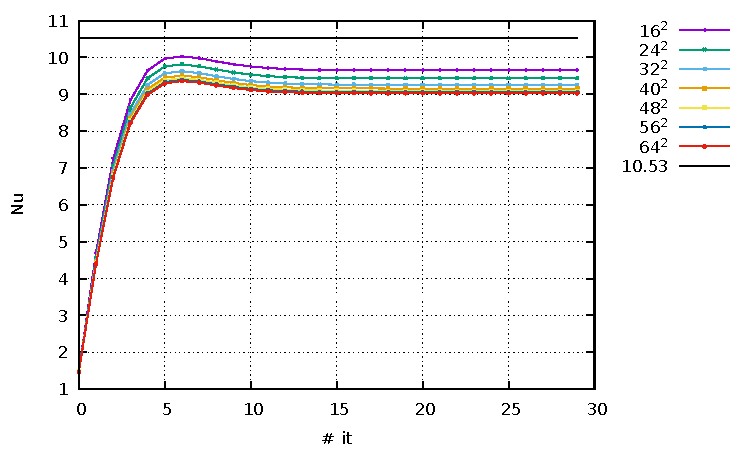
\includegraphics[width=5.7cm]{python_codes/fieldstone_110/results_EBA/Nu_Ra1e5.pdf}
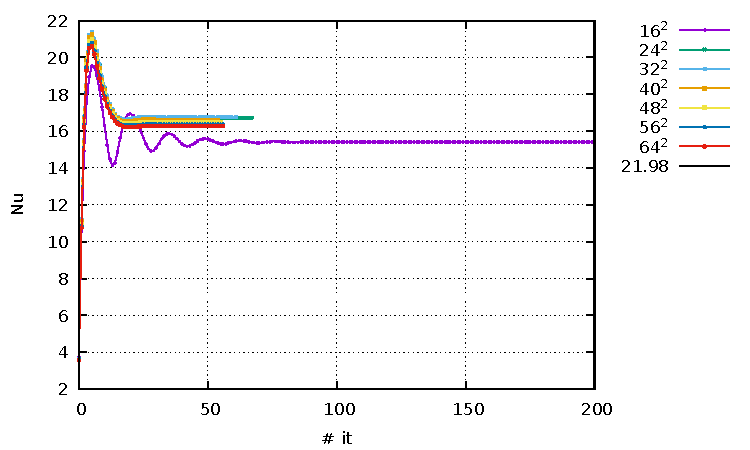
\includegraphics[width=5.7cm]{python_codes/fieldstone_110/results_EBA/Nu_Ra1e6.pdf}\\
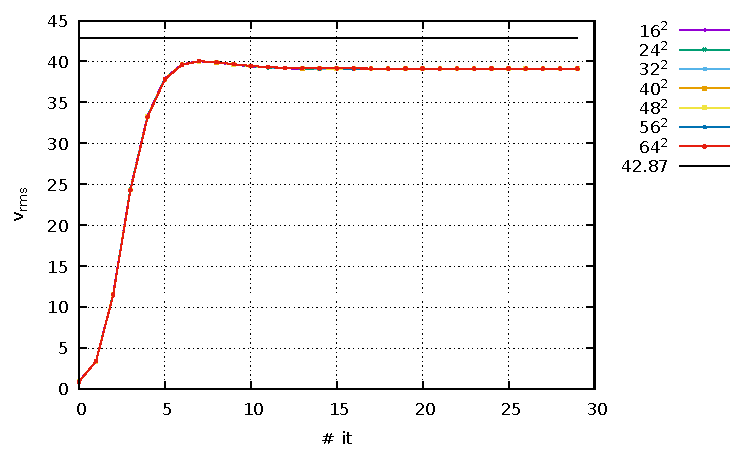
\includegraphics[width=5.7cm]{python_codes/fieldstone_110/results_EBA/vrms_Ra1e4.pdf}
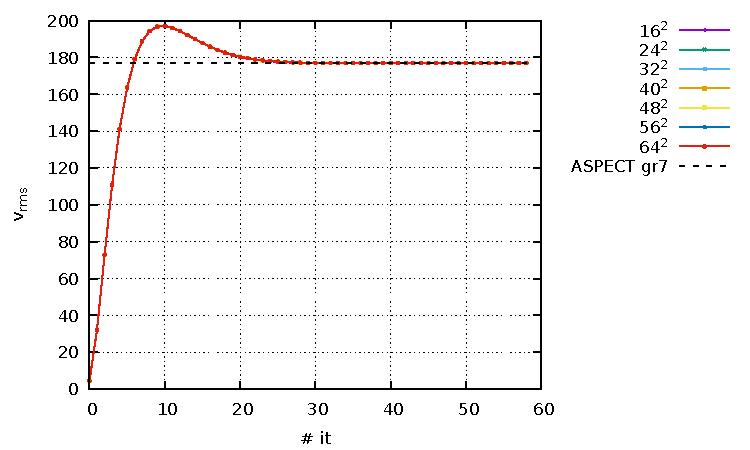
\includegraphics[width=5.7cm]{python_codes/fieldstone_110/results_EBA/vrms_Ra1e5.pdf}
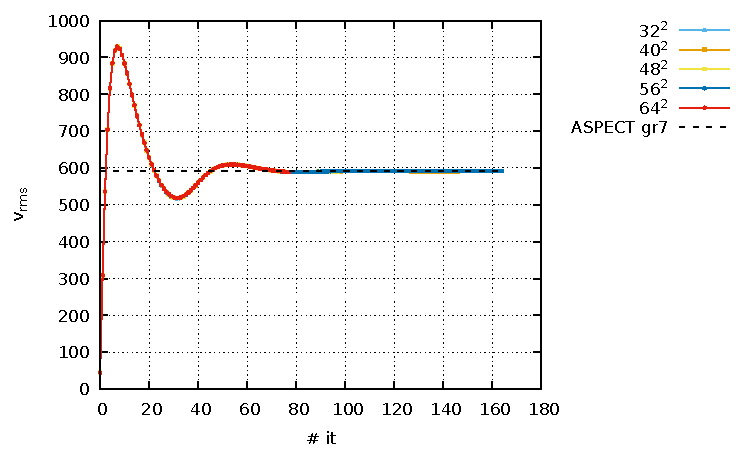
\includegraphics[width=5.7cm]{python_codes/fieldstone_110/results_EBA/vrms_Ra1e6.pdf}\\
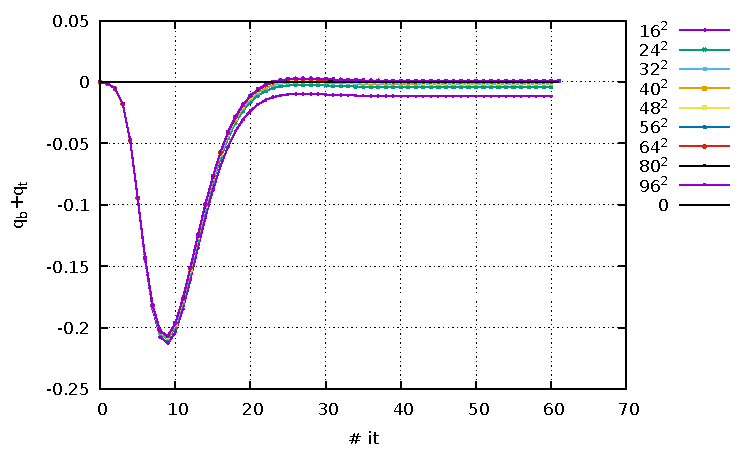
\includegraphics[width=5.7cm]{python_codes/fieldstone_110/results_EBA/q_Ra1e4.pdf}
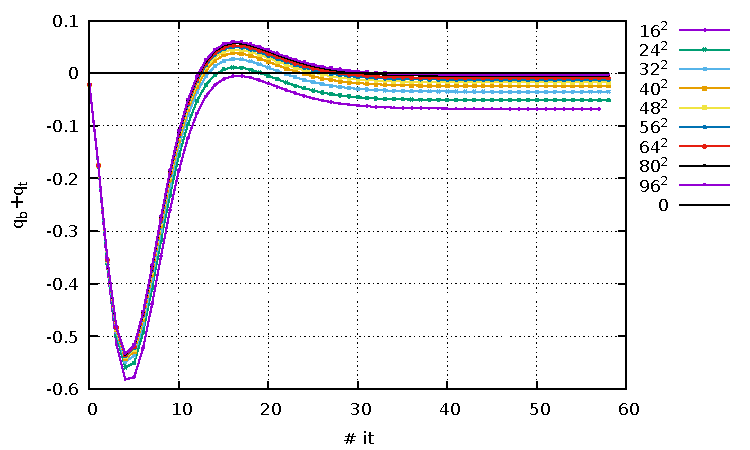
\includegraphics[width=5.7cm]{python_codes/fieldstone_110/results_EBA/q_Ra1e5.pdf}
\includegraphics[width=5.7cm]{python_codes/fieldstone_110/results_EBA/q_Ra1e6.pdf}\\
\includegraphics[width=5.7cm]{python_codes/fieldstone_110/results_EBA/T_profile_Ra1e4.pdf}
\includegraphics[width=5.7cm]{python_codes/fieldstone_110/results_EBA/T_profile_Ra1e5.pdf}
\includegraphics[width=5.7cm]{python_codes/fieldstone_110/results_EBA/T_profile_Ra1e6.pdf}\\
\includegraphics[width=5.7cm]{python_codes/fieldstone_110/results_EBA/vel_profile_Ra1e4.pdf}
\includegraphics[width=5.7cm]{python_codes/fieldstone_110/results_EBA/vel_profile_Ra1e5.pdf}
\includegraphics[width=5.7cm]{python_codes/fieldstone_110/results_EBA/vel_profile_Ra1e6.pdf}\\
\includegraphics[width=5.7cm]{python_codes/fieldstone_110/results_EBA/T_avrg_Ra1e4.pdf}
\includegraphics[width=5.7cm]{python_codes/fieldstone_110/results_EBA/T_avrg_Ra1e5.pdf}
\includegraphics[width=5.7cm]{python_codes/fieldstone_110/results_EBA/T_avrg_Ra1e6.pdf}\\
\includegraphics[width=5.7cm]{python_codes/fieldstone_110/results_EBA/conv_Ra1e4.pdf}
\includegraphics[width=5.7cm]{python_codes/fieldstone_110/results_EBA/conv_Ra1e5.pdf}
\includegraphics[width=5.7cm]{python_codes/fieldstone_110/results_EBA/conv_Ra1e6.pdf}\\
{\captionfont Left: $\Ranb=10^4$, middle: $\Ranb=10^5$, right: $\Ranb=10^6$} 
\end{center}

\begin{center}
\includegraphics[width=5.7cm]{python_codes/fieldstone_110/results_EBA/vel_1e4}
\includegraphics[width=5.7cm]{python_codes/fieldstone_110/results_EBA/vel_1e5}
\includegraphics[width=5.7cm]{python_codes/fieldstone_110/results_EBA/vel_1e6}\\
\includegraphics[width=5.7cm]{python_codes/fieldstone_110/results_EBA/T_1e4}
\includegraphics[width=5.7cm]{python_codes/fieldstone_110/results_EBA/T_1e5}
\includegraphics[width=5.7cm]{python_codes/fieldstone_110/results_EBA/T_1e6}\\
\includegraphics[width=5.7cm]{python_codes/fieldstone_110/results_EBA/q_1e4}
\includegraphics[width=5.7cm]{python_codes/fieldstone_110/results_EBA/q_1e5}
\includegraphics[width=5.7cm]{python_codes/fieldstone_110/results_EBA/q_1e6}\\
\includegraphics[width=5.7cm]{python_codes/fieldstone_110/results_EBA/sh_1e4}
\includegraphics[width=5.7cm]{python_codes/fieldstone_110/results_EBA/sh_1e5}
\includegraphics[width=5.7cm]{python_codes/fieldstone_110/results_EBA/sh_1e6}\\
\includegraphics[width=5.7cm]{python_codes/fieldstone_110/results_EBA/adiab_1e4}
\includegraphics[width=5.7cm]{python_codes/fieldstone_110/results_EBA/adiab_1e5}
\includegraphics[width=5.7cm]{python_codes/fieldstone_110/results_EBA/adiab_1e6}\\
{\captionfont Left: $\Ranb=10^4$, middle: $\Ranb=10^5$, right: $\Ranb=10^6$}\\
probably slight bug in shear heating values.redo 
\end{center}

\newpage
\aspect results for 16x16, 32x32, 64x64 meshes

\begin{center}
\includegraphics[width=5.7cm]{python_codes/fieldstone_110/results_EBA/aspect/vrms_1e4}
\includegraphics[width=5.7cm]{python_codes/fieldstone_110/results_EBA/aspect/vrms_1e5}
\includegraphics[width=5.7cm]{python_codes/fieldstone_110/results_EBA/aspect/vrms_1e6}\\
\includegraphics[width=5.7cm]{python_codes/fieldstone_110/results_EBA/aspect/qsum_1e4}
\includegraphics[width=5.7cm]{python_codes/fieldstone_110/results_EBA/aspect/qsum_1e5}
\includegraphics[width=5.7cm]{python_codes/fieldstone_110/results_EBA/aspect/qsum_1e6}\\
\includegraphics[width=5.7cm]{python_codes/fieldstone_110/results_EBA/aspect/qtop_1e4}
\includegraphics[width=5.7cm]{python_codes/fieldstone_110/results_EBA/aspect/qtop_1e5}
\includegraphics[width=5.7cm]{python_codes/fieldstone_110/results_EBA/aspect/qtop_1e6}\\
{\captionfont Left: $\Ranb=10^4$, middle: $\Ranb=10^5$, right: $\Ranb=10^6$} 
\end{center}

\vspace{5mm}

\begin{center}
\begin{tabular}{llcccccc}
\hline
$\Ranb$  &  &\aspect  &\aspect  & \aspect & \stone 110  & \stone 110 & \stone 110\\
         &  &(16x16)  & (32x32) & (64x64) & (32x32)     & (64x64)    & (80x80) \\
\hline
\hline
$10^4$ & $\upnu_{rms}$ &     & 39.159131    & 39.1590718  &  39.1220715117  & 39.1427811339 & 39.1469649726 \\
       & $q_{bot}$     &     & -4.21461224  & -4.21459920 &  -4.2526699758  & -4.2241736047 & -4.2207111697 \\
       & $q_{top}$     &     & +4.21466572  & +4.21465118 &  +4.2561018386  & 4.2260501790  & 4.2223536559  \\  
\hline
$10^5$ & $\upnu_{rms}$ &     & 176.8339244  & 176.7353244 &  176.3717700756 & 176.6073765137& 176.6555842304 \\
       & $q_{bot}$     &     & -8.93023781  & -8.90386799 & -9.2311968388   & -9.0088339160 & -8.9775516981  \\ 
       & $q_{top}$     &     & +8.93021403  & +8.90519202 & +9.2584172686   & 9.0239878253  & +8.9908296677  \\
\hline
$10^6$ & $\upnu_{rms}$ &     & 590.707916   & 591.340132  &  556.3611676986 & 570.1830724535&  \\
       & $q_{bot}$     &     & -15.9490236  & -16.0182326 & -16.1081289993  & -16.1217624933&  \\
       & $q_{top}$     &     & +15.9661980  & +16.0184006 & +16.7479398662  & 16.2626758191 &  \\ 
\hline
\end{tabular}
\end{center}

At high Rayleigh numbers the $v_{rms}$ values are still 3\% off.
I should rerun stone and make sure it did reach steady state. 

Also the velocity profiles are somewhat off still. 


